\PassOptionsToClass{fontset=fandol}{ctexart}
\documentclass{rjthesis}
\usepackage{booktabs}
\usepackage{amsmath}
\usepackage{graphicx}
\usepackage{array}
\usepackage{float}
\usepackage{makecell}
\usepackage{bbm}
\usepackage{amssymb}
\usepackage[backend=biber,style=numeric,sorting=none,giveninits=true,defernumbers=true]{biblatex}
\addbibresource{references.bib}

\defbibheading{rjrefs}{\section*{#1}}
\defbibheading{rjcnrefs}{%
	\par\vspace{8pt}
	{\xiaowuhao\noindent \textbf{#1}\par}
}
\AtBeginBibliography{\rjbibfont}
\setlength{\bibitemsep}{0pt}

\rjhead{高宇岑 等:基于多模态数据融合的下一兴趣点推荐}

\rjtitle{基于多模态数据融合的下一兴趣点推荐方法\textsuperscript{*}}
\rjauthor{高宇岑\textsuperscript{1}, 王雪凝\textsuperscript{2}, 庄新鱼\textsuperscript{2}, 王斌\textsuperscript{2}, 杨晓春\textsuperscript{1}}
\rjinfor{\textsuperscript{1}(东北大学软件学院, 沈阳, 110169)\\
\textsuperscript{2}(东北大学计算机学院, 沈阳, 110169)\\
通讯作者: 杨晓春, E-mail: yangxc@mail.neu.edu.cn
}
\rjabstracttext{下一兴趣点(Point-of-Interest, POI)推荐是位置服务、城市计算与智能出行中的基础问题,其目标是根据用户历史签到序列预测下一次访问地点.与一般序列推荐不同,该任务同时涉及转移拓扑、地理空间、时间节律和地点语义等多源异构信息,本质上属于面向城市兴趣点对象的多模态数据建模与融合问题.现有方法通常围绕单一模态或弱耦合的时空特征展开建模,对POI文本语义、结构连通性与上下文依赖之间的协同关系利用不足;同时,不同模态来源、粒度和统计分布差异显著,直接拼接或固定权重融合难以充分弥合表示空间鸿沟.本文提出一种Path-LLM风格的下一POI多模态表示学习框架,将拓扑、语义、空间、时间以及用户上下文统一纳入序列建模流程.框架包含三个核心组成:(1) 跨模态对齐模块SemAlign,通过实例级与特征级InfoNCE损失将POI的拓扑表示与语义表示映射到共享空间;(2) 上下文感知门控融合模块ContextFusion,依据当前序列上下文和用户画像自适应调节拓扑与语义信息的融合权重,并结合空间和时间模态构造多模态POI token;(3) 选择性微调GPT-2骨干网络,利用预训练自回归序列结构完成下一POI预测,并可进一步叠加由训练集构建的统计先验增强候选排序.在NYC签到数据集上的实验表明,纯神经模型在HR@10和NDCG@10上分别达到37.66\%和24.28\%,结合统计先验后进一步提升至47.12\%和30.70\%.进一步的消融和分析实验表明,时间模态、跨模态对齐和上下文自适应融合均对性能提升具有独立贡献.本文为多模态数据管理与融合场景下的POI推荐提供了一种结构清晰、可解释且可扩展的建模范式.}
\rjkeywords{多模态数据融合; 下一兴趣点推荐; POI表示学习; 预训练序列模型; 跨模态对齐; 自适应融合}
\rjclc{TP391}
\rjcncite{高宇岑,王雪凝,庄新鱼,王斌,杨晓春.基于多模态数据融合的下一兴趣点推荐方法.软件学报,20XX,XX(XX):1--XX. http://www.jos.org.cn/1000-9825/0000.htm}
\rjencite{Gao YC, Wang XN, Zhuang XY, Wang B, Yang XC. Next point-of-interest recommendation via multi-modal data fusion. Ruan Jian Xue Bao/Journal of Software, 20XX,XX(XX):1--XX (in Chinese). http://www.jos.org.cn/1000-9825/0000.htm}
\rjetitle{Next Point-of-Interest Recommendation via Multi-Modal Data Fusion}
\rjeauthor{GAO Yu-Cen\textsuperscript{1}, WANG Xue-Ning\textsuperscript{2}, ZHUANG Xin-Yu\textsuperscript{2}, WANG Bin\textsuperscript{2}, YANG Xiao-Chun\textsuperscript{1}}
\rjeinfor{\textsuperscript{1}(Software College, Northeastern University, Shenyang 110169, China)\\
\textsuperscript{2}(School of Computer Science and Engineering, Northeastern University, Shenyang 110169, China)}
\rjeabstracttext{Next Point-of-Interest (POI) recommendation is a fundamental task in location-based services, urban computing, and intelligent mobility, aiming to predict a user's next visit from historical check-in sequences. Different from general sequential recommendation, this task jointly involves transition topology, geographic space, temporal rhythm, and POI semantics, and is therefore essentially a multi-modal urban data modeling and fusion problem. Existing methods usually rely on a single modality or loosely coupled spatiotemporal features, which are insufficient for capturing the heterogeneous nature of POIs and the representation gap across modalities. This paper presents a Path-LLM-style multi-modal POI representation learning framework that integrates topology, semantics, space, time, and user context into a unified sequential modeling architecture. The framework contains three key components: (1) SemAlign, a cross-modal alignment module that maps topological and semantic POI representations into a shared space via instance-level and feature-level InfoNCE objectives; (2) ContextFusion, an adaptive context-aware gating mechanism that dynamically balances topological and semantic signals conditioned on trajectory context and user profiles and further incorporates spatial and temporal modalities to construct multi-modal POI tokens; and (3) a selectively fine-tuned GPT-2 backbone that leverages pretrained autoregressive sequential structures for next-POI prediction, with optional training-only statistical priors for enhanced candidate ranking. Experiments on the NYC check-in dataset show that the pure neural model achieves 37.66\% HR@10 and 24.28\% NDCG@10, and the statistical-prior-enhanced version further improves them to 47.12\% and 30.70\%. Further ablation and analytical results verify the contributions of temporal modality, cross-modal alignment, and adaptive fusion. The proposed framework provides a clear, interpretable, and extensible modeling paradigm for POI recommendation under multi-modal data management and fusion scenarios.}
\rjekeywords{multimodal data fusion; next POI recommendation; POI representation learning; pretrained sequential model; cross-modal alignment; adaptive fusion}
\rjauthorsbio{
\noindent \textbf{高宇岑}，副教授，硕士生导师，主要研究领域为数据工程与优化算法.\\
\textbf{王雪凝}，博士研究生，主要研究领域为时空数据管理与智能推荐.\\
\textbf{庄新鱼}，硕士研究生，主要研究领域为多模态学习与数据挖掘.\\
\textbf{王\quad 斌}，博士，教授，博士生导师，CCF专业会员，主要研究领域为数据管理与智能系统.\\
\textbf{杨晓春}，博士，教授，博士生导师，CCF杰出会员，主要研究领域为数据库、数据管理与智能信息处理.}

\begin{document}

\rjmaketitle

\section{引言}

基于位置的社交网络(location-based social networks, LBSNs)如Foursquare、Yelp和大众点评等平台的广泛普及,积累了海量的用户签到数据.这些数据记录了用户与城市兴趣点(Point-of-Interest, POI)之间的交互行为,为个性化下一跳POI推荐服务提供了重要的数据基础\cite{zheng2015trajectory,zhang2021survey}.与传统的序列推荐(如电影或商品推荐)不同,下一POI推荐直接面向城市空间中的实体对象,既要刻画用户偏好,又要理解地点之间的转移关系、地理约束和语义功能差异,因此天然具有时空异构、多模态融合和强上下文依赖的特点.

从数据视角看,下一POI推荐并不是单纯的序列预测任务,而是一个典型的多模态数据管理与融合问题.一方面,POI本身同时具有图结构连通性、地理坐标、类别标签和文本语义等异构属性;另一方面,用户轨迹又引入了显式的时间顺序、周期性行为和跨区域迁移模式.这些模态在粒度、噪声水平、稀疏性和更新频率上均存在显著差异:例如,转移拓扑依赖历史行为统计,文本语义来自相对静态的元数据描述,空间坐标具有连续度量结构,而时间模态则反映用户活动节律.如何在统一框架中实现不同模态的组织、对齐、融合与下游推荐,是多模态POI推荐研究中的关键问题.

早期下一POI推荐方法\cite{luo2021stan,yang2022getnext}主要依赖于循环神经网络或自注意力机制对签到序列进行建模,并将空间和时间信息作为辅助特征注入.这类方法推动了时空序列建模的发展,但通常仍将POI压缩为单一嵌入向量,对地点语义、转移结构和上下文依赖之间的协同关系刻画不足.近年来,大语言模型(large language models, LLMs)\cite{brown2020language,devlin2019bert}的成功激发了研究者利用预训练语言模型进行轨迹理解.在路径表示学习领域,已有工作通过对比学习对齐拓扑和语义模态\cite{wei2025pathllm},展示了多模态融合在移动性任务中的潜力.多模态表示学习在视觉--语言理解等跨领域任务中同样取得了显著进展\cite{radford2021clip},为将POI文本语义与结构信息联合建模提供了借鉴.

尽管如此,现有工作在多模态融合方面仍面临三个关键挑战.首先,POI的拓扑、语义、空间和时间信息来自不同数据源,其表示粒度和统计分布差异显著,直接融合容易造成模态语义错位.特别是拓扑模态强调用户行为中的转移连通性,语义模态强调地点功能和类别相似性,二者虽然互补,却天然处于不同表示空间.其次,用户移动行为具有强上下文依赖,在通勤、消费、娱乐和跨区域移动等不同场景下,各模态的重要性会动态变化,固定权重融合或简单拼接难以适应这种轨迹上下文差异.再次,预训练序列模型为轨迹建模提供了强大的自回归建模结构,但如何将异构POI属性组织为适合序列骨干处理的多模态token,并在有限签到数据上实现有效适配,仍需要专门设计.

针对上述问题,本文提出一种多模态POI表示学习框架.该框架将POI建模为四种明确的模态:拓扑模态(图结构嵌入与转移图特征)、语义模态(文本描述与类别嵌入)、空间模态(GPS坐标)和时间模态(签到时刻与时间间隔).在此基础上,本文设计了三项核心机制:(1) SemAlign跨模态对齐模块,通过实例级和特征级InfoNCE损失将拓扑和语义表示对齐到统一的共享空间,缓解异构模态表示空间不一致问题;(2) ContextFusion自适应上下文门控融合机制,根据序列上下文动态调节拓扑和语义特征的融合权重,克服固定融合策略对移动场景变化适应性不足的问题;(3) 选择性微调GPT-2骨干网络,仅更新位置嵌入和层归一化参数,利用预训练自回归序列结构完成多模态POI token的序列建模与下一POI预测.

与侧重候选空间约束或轨迹语言化推理的工作不同,本文关注POI对象自身的多模态表示组织、跨模态对齐与上下文自适应融合问题.这些机制与候选生成、重排序和用户协同建模具有互补性:一方面,高质量的多模态POI表示能够提升全空间匹配和候选重排序的判别能力;另一方面,上下文感知的融合权重也为解释不同轨迹场景下的推荐依据提供了可分析信号.因此,本文从多模态数据管理与融合视角出发,系统研究四类POI模态如何被统一组织、显式对齐并服务于下一POI推荐.

本文的主要贡献如下.
\begin{enumerate}
	\item 提出四种显式模态编码器(拓扑、语义、空间、时间),将POI的多模态特性系统性地纳入统一的表示学习框架.
	\item 设计SemAlign跨模态对齐模块,通过实例级和特征级InfoNCE损失的双层对齐策略,实现拓扑与语义模态之间的语义一致性.
	\item 提出ContextFusion自适应上下文门控融合机制,使模型能够根据当前序列上下文动态调节模态融合权重,克服固定融合策略的局限.
	\item 在纽约市签到数据集上进行的实验表明,纯神经模型在HR@10和NDCG@10上分别达到37.66\%和24.28\%,结合统计先验后进一步提升至47.12\%和30.70\%,并通过消融实验、门控行为分析和泛化分析验证了各设计模块的有效性与可解释性.
\end{enumerate}

\section{相关工作}

\subsection{下一POI推荐}

下一POI推荐旨在根据用户的历史签到序列预测用户下一次将访问的位置.早期工作\cite{zheng2015trajectory}主要基于马尔可夫链和矩阵分解.随着深度学习的发展,基于RNN的模型\cite{luo2021stan}被引入以捕获序列依赖关系,随后基于自注意力的架构\cite{kang2018sasrec,sun2019bert4rec}进一步扩展了长距离交互建模能力.近期方法通过多种编码方案集成空间和时间上下文\cite{yang2022getnext,liu2021stgcn}.例如,GETNext\cite{yang2022getnext}通过轨迹流图增强Transformer进行下一POI推荐;MTNet\cite{mtnet}利用移动性树学习时间槽偏好.这些方法大多将POI表示为单一特征向量,未能利用城市地点的多面性.

在轨迹数据管理领域,研究者关注移动对象位置序列的存储、索引和查询分析.随着GPS设备的普及,轨迹数据规模迅速增长,系统需要同时处理空间邻近性、时间顺序和移动语义\cite{zheng2015trajectory}.在智能推荐场景中,POI表示学习进一步将原始签到序列转化为低维向量,以支持下一跳推荐等下游任务.

近年来,对比学习在序列推荐中展现出潜力.DuoRec\cite{duoRec}采用对比正则化重构序列表示分布,TiCoSeRec\cite{dang2023ticosec}引入时间间隔感知的数据增强策略.在图像增强与序列建模方面,MAERec\cite{maerec}利用图掩码自编码器进行序列推荐,CrossDR\cite{crossdr}探索跨域表示解耦.此外,扩散模型也被引入序列推荐领域,DiffuRec\cite{diffuRec}利用扩散过程建模推荐中的不确定性和多样性.然而,现有方法对POI多模态信息的利用仍显不足.

\subsection{大语言模型与多模态表示学习}

多模态学习在视觉-语言理解等不同领域已取得显著成功\cite{radford2021clip}.大语言模型在文本理解、序列建模和少样本泛化方面表现突出\cite{brown2020language,devlin2019bert}.由于POI名称、类型、类别描述和区域功能都可以自然转化为文本,近年来研究者开始将语言模型引入POI推荐领域.在路径表示学习领域,Path-LLM\cite{wei2025pathllm}将道路拓扑嵌入与道路文本语义纳入统一框架,通过对比学习对齐两种模态,验证了跨模态对齐在移动性任务中的有效性.本文在此基础上进一步引入空间和时间模态,以应对POI推荐中特有的空间邻近性和时间周期性需求,形成更完整的POI多模态表示框架.

值得注意的是,近期LLM驱动的POI推荐研究开始关注“轨迹到语言”的转换与候选空间约束.CoMaPOI\cite{comapoi}通过Profiler、Forecaster和Predictor三个协同代理,分别承担数值时空信息语言化、候选集合动态收缩和最终预测的功能,展示了语言化轨迹理解和候选空间管理在下一POI推荐中的作用.与此类方法相比,本文关注另一条互补路径:从POI对象自身出发,研究拓扑、语义、空间和时间等异构模态如何被统一编码、显式对齐并基于轨迹上下文自适应融合.这种多模态表示学习能力可为后续候选生成、重排序或轨迹画像增强提供更具判别性的基础表示.

\subsection{跨模态对齐与自适应融合}

跨模态对齐是多模态学习中的核心问题之一.对比学习框架如CLIP\cite{radford2021clip}通过对齐图像和文本的嵌入空间实现了卓越的零样本泛化能力.本文在该方向上的设计包含两层:首先通过实例级对齐学习区分不同POI的判别性特征,再通过特征级对齐促进模态间的子空间一致性.在融合策略方面,现有方法多采用固定权重的拼接或加法融合.本文提出的ContextFusion通过序列上下文感知的门控机制动态调节融合权重,使模型能够根据当前序列上下文自适应地权衡各模态信息的贡献.

从数据融合角度看,跨模态对齐与融合并非简单的特征堆叠问题.对于下一POI推荐任务,拓扑模态强调“去过哪些地方之后通常会去哪里”,语义模态强调“哪些地点在功能上相似”,空间模态强调“哪些地点在物理上可达”,时间模态则强调“在何时何地更可能发生访问行为”.这些模态之间既互补又可能产生冲突:例如,两个语义相似的咖啡馆可能在空间上相距很远,而两个空间相近的POI在功能上可能完全不同.因此,如何在保持模态判别性的同时学习跨模态的一致性,并让融合过程对上下文敏感,是本文方法设计的出发点.

\section{问题定义}

本文研究LBSN场景下的下一兴趣点(Point-of-Interest, POI)推荐问题.设用户集合为$\mathcal{U}=\{u_1,u_2,\ldots,u_N\}$,POI集合为$\mathcal{P}=\{p_1,p_2,\ldots,p_M\}$.每个POI $p_j\in\mathcal{P}$具有相应的地理位置$\mathbf{g}_j=(lat_j,lng_j)$、类别信息$c_j\in\mathcal{C}$,并可关联名称、描述等文本语义信息.用户$u$在时间$t_i$对POI $p_i$的一次访问行为定义为签到记录:
\begin{equation}
	x_i^u=(u,p_i,t_i).
\end{equation}

对于用户$u$,将其历史签到记录按照时间顺序排列,得到用户历史访问轨迹:
\begin{equation}
	\mathcal{H}_u^{(n)}=[x_1^u,x_2^u,\ldots,x_n^u],\quad t_1<t_2<\cdots<t_n,
\end{equation}
其中,$\mathcal{H}_u^{(n)}$表示用户$u$截至当前时刻的历史访问序列.

在多模态POI推荐场景中,除历史访问轨迹外,任务还可以利用与用户轨迹和候选POI相关的可用上下文信息.本文用$\mathbf{m}_u^{(n)}$表示用户$u$历史轨迹中的多模态上下文,其可包括POI地理位置、类别属性、文本语义、签到时间以及由历史访问行为形成的转移关系等信息.这些信息均作为下一POI推荐任务的可用输入,用于描述用户访问行为及候选POI的上下文属性.

\textbf{下一POI推荐任务}旨在根据用户$u$的历史访问轨迹$\mathcal{H}_u^{(n)}$、可用的多模态上下文$\mathbf{m}_u^{(n)}$以及候选POI集合$\mathcal{P}$,预测用户在下一时刻最可能访问的POI $p_{n+1}$.任务输出为候选POI上的排序结果,并返回Top-$K$推荐列表:
\begin{equation}
	\mathcal{R}_u^K=[p_{r_1},p_{r_2},\ldots,p_{r_K}],\quad p_{r_i}\in\mathcal{P}.
\end{equation}

该任务的目标是使用户真实访问的下一POI $p_{n+1}$在推荐列表$\mathcal{R}_u^K$中获得尽可能高的排名.

\section{模型方法}

\begin{figure}[t]
	\centering
	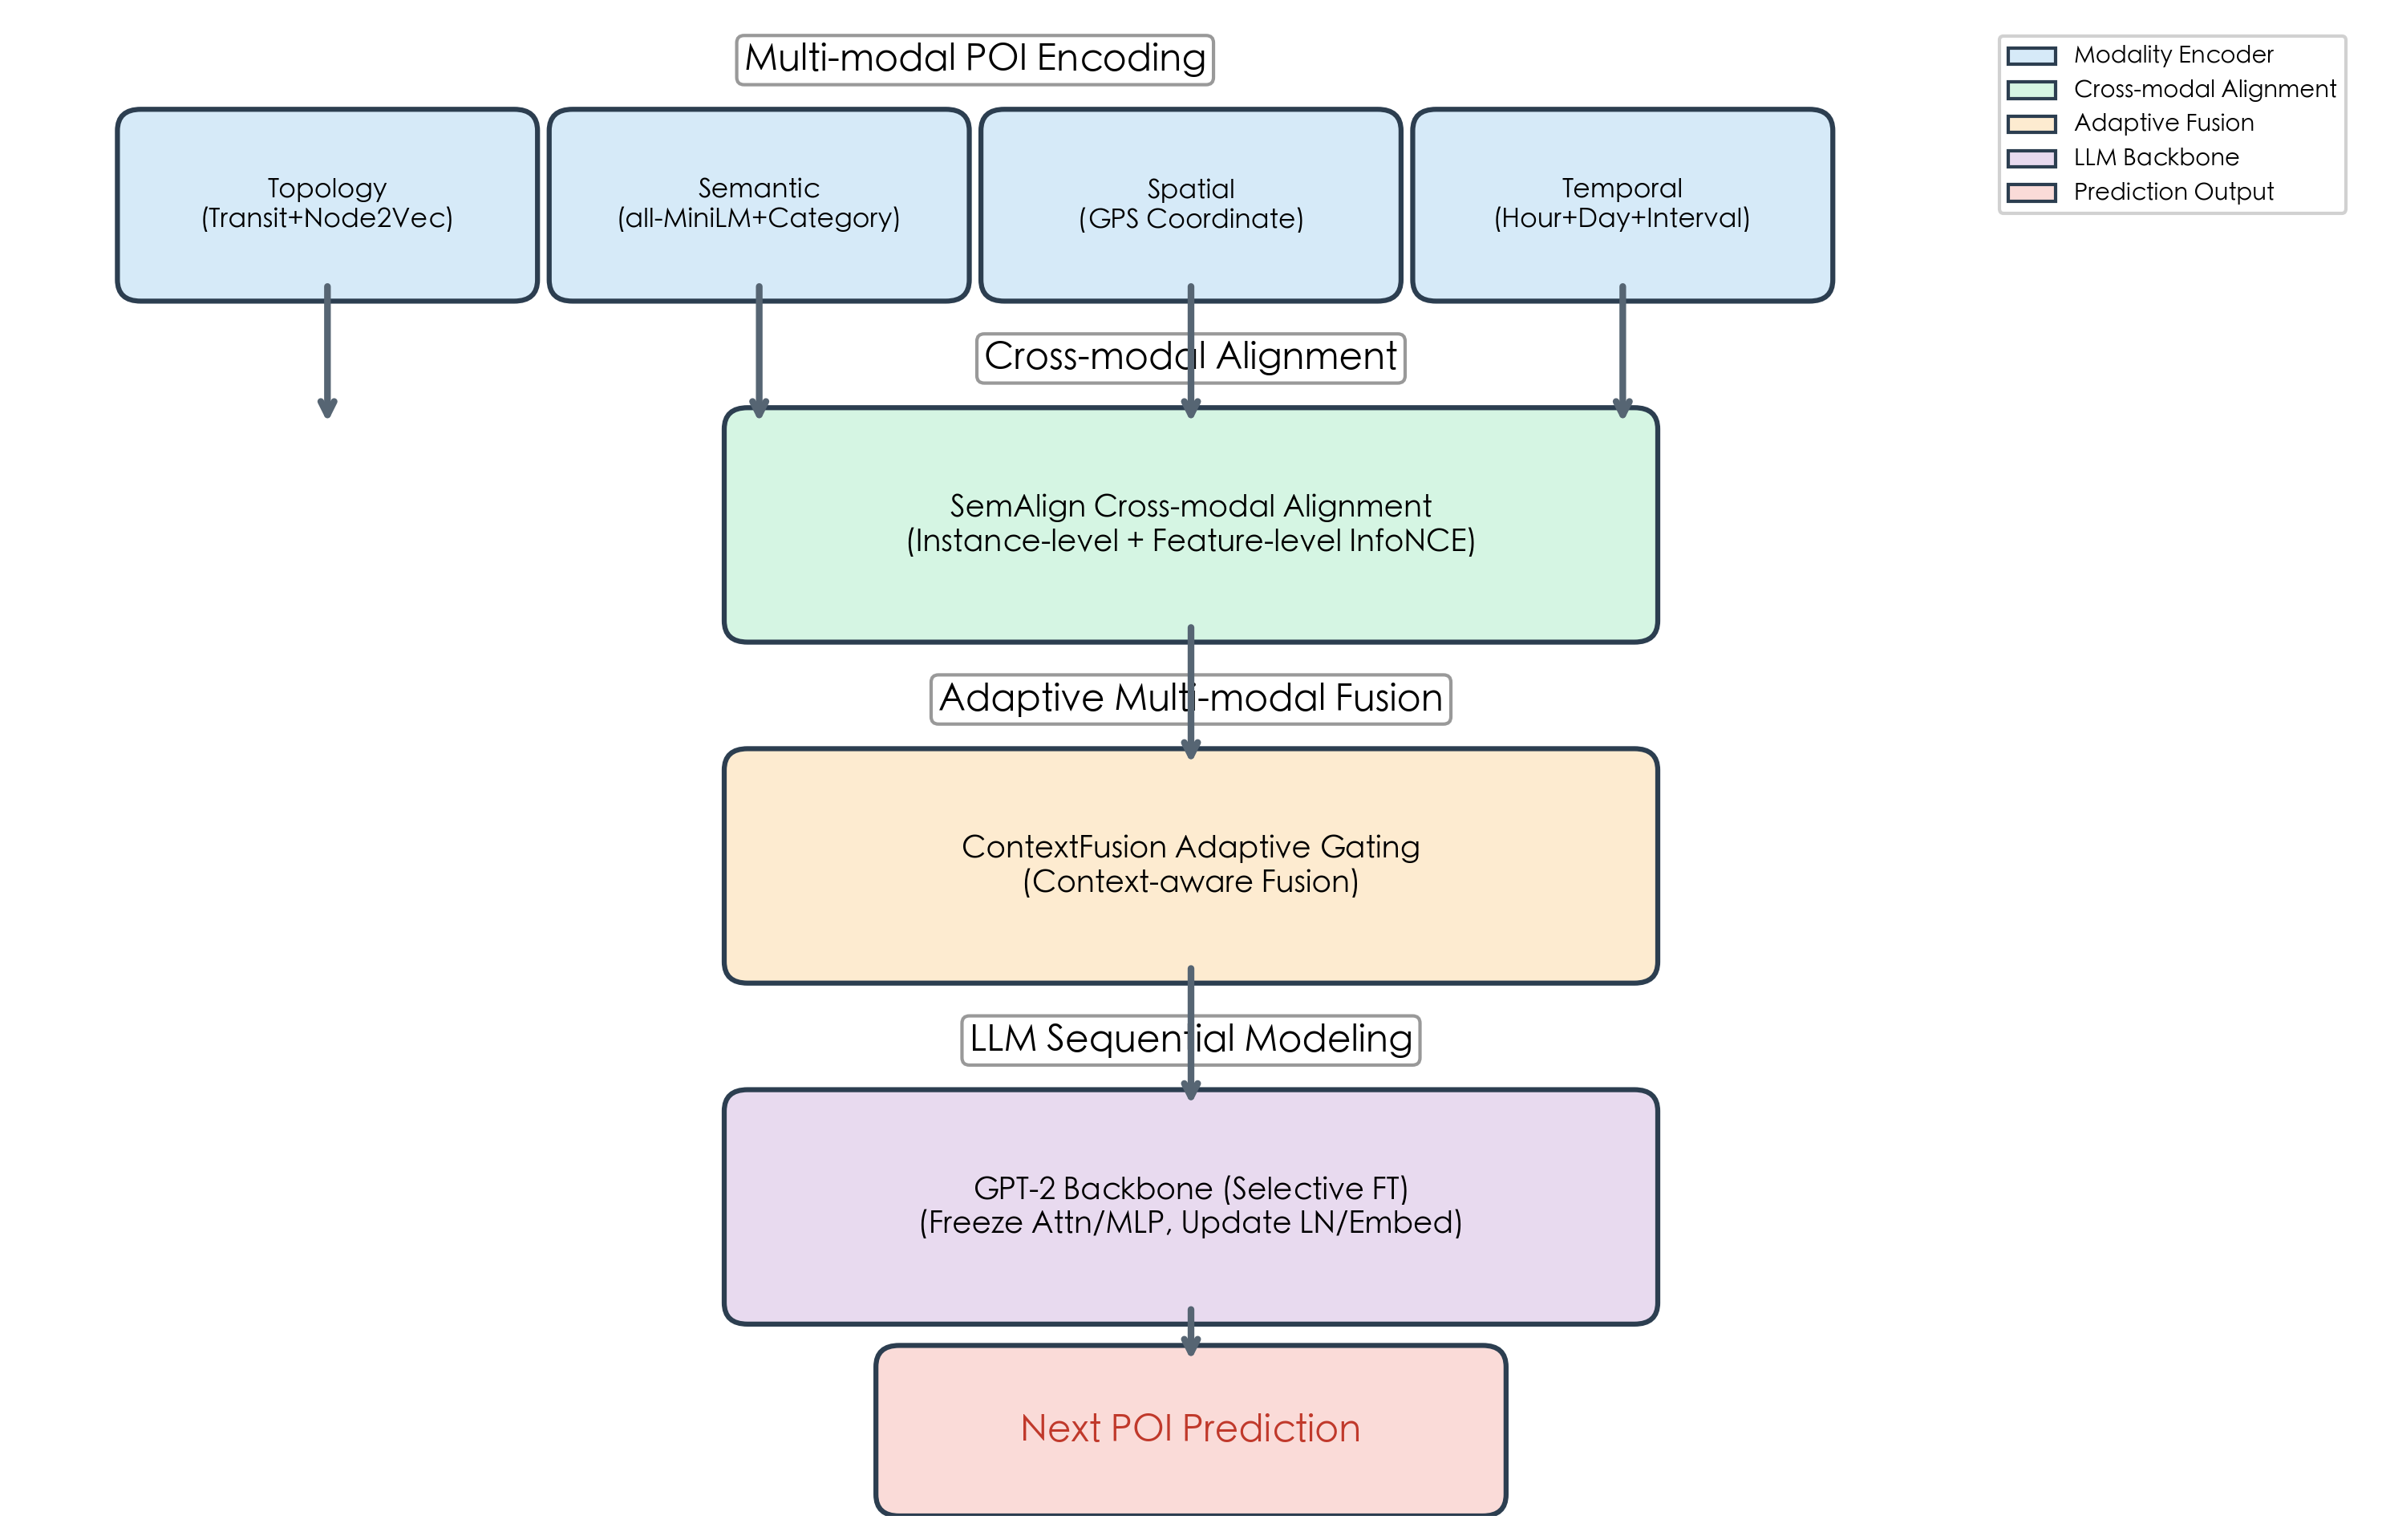
\includegraphics[width=0.98\linewidth]{figure/framework.png}
	\caption{多模态POI推荐框架总体架构}
	\label{fig:framework}
\end{figure}

本文提出的多模态POI推荐框架总体架构如图~\ref{fig:framework}所示.模型遵循Path-LLM风格的“对象多模态编码--跨模态对齐--上下文融合--序列预测”流程,包含五个主要阶段:(1) 多模态POI与用户上下文编码,(2) 跨模态对齐(SemAlign),(3) 自适应上下文融合(ContextFusion),(4) 基于选择性微调GPT-2的序列建模,以及(5) 查询向量与候选POI向量的归一化匹配.在扩展设置中,模型还可叠加仅由训练集构建的流行度、转移、重复访问、用户偏好和空间邻近等统计先验,用于增强最终候选排序.每个阶段的详细设计如下.

\subsection{多模态POI编码}

\subsubsection{拓扑编码器}

拓扑模态捕获POI之间的结构关系.我们从训练集中构造有向加权转移图$\mathcal{G}_t$,其中边权重$w_{ij}$表示从POI $i$转移到POI $j$的频率.对于每个POI,提取转移特征向量(入度、出度、PageRank、转移概率)和Node2Vec\cite{grover2016node2vec}嵌入.拓扑编码器将两种特征投影到$d$维隐藏空间:
\begin{equation}
	\mathbf{h}_p^{\text{topo}}=\text{LayerNorm}(\text{MLP}_{\text{feat}}(\mathbf{f}_p)+\text{MLP}_{\text{n2v}}(\mathbf{e}_p))\cdot\mathbbm{1}_{\text{avail}}(p),
	\label{eq:topo_encoder}
\end{equation}
其中$\mathbbm{1}_{\text{avail}}(p)$是训练数据充足的POI指示函数.

\subsubsection{语义编码器}

语义模态捕获POI的文本和类别属性.使用预训练句子嵌入模型(all-MiniLM-L6-v2)将POI文本描述编码为384维嵌入,然后投影到$d$维空间.类别信息通过可学习的类别嵌入表引入:
\begin{equation}
	\mathbf{h}_p^{\text{sem}}=\text{LayerNorm}(\mathbf{W}_{\text{text}}\cdot\text{all-MiniLM}(text_p)+\mathbf{E}_{\text{cat}}(c_p)).
	\label{eq:sem_encoder}
\end{equation}

\subsubsection{空间编码器}

空间模态利用GPS坐标建模地理邻近性.坐标经归一化后通过两层MLP(激活函数为GELU)投影到$d$维空间:
\begin{equation}
	\mathbf{h}_p^{\text{spat}}=\text{MLP}_{\text{coord}}([lat_p,lng_p]).
	\label{eq:spat_encoder}
\end{equation}

\subsubsection{时间编码器}

时间模态捕获用户签到行为的周期性模式.对每次签到事件,提取三个时间特征:小时(hour-of-day, 0--23)、星期(day-of-week, 0--6)和时间间隔桶(log-scaled time-interval bucket, 8个桶).每种特征通过独立的嵌入表编码并求和:
\begin{equation}
	\mathbf{h}_t^{\text{temp}}=\text{LayerNorm}(\mathbf{E}_{\text{hour}}(h_t)+\mathbf{E}_{\text{wkd}}(w_t)+\mathbf{E}_{\text{del}}(\delta_t)).
	\label{eq:temp_encoder}
\end{equation}

\subsubsection{用户上下文与画像编码器}

除POI自身属性外,下一POI推荐还需要刻画用户长期偏好.本文将用户ID嵌入与用户类别画像作为辅助上下文.其中,用户类别画像由训练集中用户访问不同POI类别的频率统计得到,再经线性投影映射到$d$维空间:
\begin{equation}
	\mathbf{h}_u^{\text{prof}}=\text{LayerNorm}(\mathbf{W}_{\text{prof}}\mathbf{r}_u),\quad
	\mathbf{h}_u^{\text{id}}=\mathbf{E}_{\text{user}}(u),
	\label{eq:user_profile}
\end{equation}
其中$\mathbf{r}_u$表示用户$u$在训练集上的类别偏好分布.为避免信息泄漏,转移图、Node2Vec、流行度、用户--POI偏好和用户--类别偏好等所有行为统计特征均仅由训练集构建,不使用验证集或测试集目标信息.

\subsection{SemAlign: 语义-拓扑跨模态对齐}

拓扑和语义特征捕获了POI互补的方面——拓扑反映结构连通性,语义反映功能相似性.为弥合两种模态之间的语义鸿沟,本文提出SemAlign,一个由两个投影头和双层InfoNCE损失组成的跨模态对齐模块.

每个POI的拓扑和语义嵌入通过MLP投影头映射到共享的对齐空间:
\begin{equation}
	\mathbf{z}_p^{\text{topo}}=\text{Proj}_{\text{topo}}(\mathbf{h}_p^{\text{topo}}),\quad
	\mathbf{z}_p^{\text{sem}}=\text{Proj}_{\text{sem}}(\mathbf{h}_p^{\text{sem}}).
	\label{eq:projection}
\end{equation}

\subsubsection{实例级对齐}

实例级InfoNCE损失将每个POI视为一个不同的类别,学习匹配其拓扑和语义视角:
\begin{equation}
	\mathcal{L}_{\text{instance}}=-\frac{1}{2N}\sum_{i=1}^N
	\left[
	\log\frac{\exp(\mathbf{z}_i^{\text{topo}}\cdot\mathbf{z}_i^{\text{sem}}/\tau)}
	{\sum_j\exp(\mathbf{z}_i^{\text{topo}}\cdot\mathbf{z}_j^{\text{sem}}/\tau)}
	+\log\frac{\exp(\mathbf{z}_i^{\text{sem}}\cdot\mathbf{z}_i^{\text{topo}}/\tau)}
	{\sum_j\exp(\mathbf{z}_i^{\text{sem}}\cdot\mathbf{z}_j^{\text{topo}}/\tau)}
	\right].
	\label{eq:instance_loss}
\end{equation}

\subsubsection{特征级对齐}

特征级InfoNCE损失对特征维度进行对齐,鼓励两种模态共享共同的潜在子空间:
\begin{equation}
	\mathcal{L}_{\text{feature}}=-\frac{1}{2d}\sum_{k=1}^d
	\left[
	\log\frac{\exp(\tilde{\mathbf{z}}_k^{\text{topo}}\cdot\tilde{\mathbf{z}}_k^{\text{sem}}/\tau)}
	{\sum_l\exp(\tilde{\mathbf{z}}_k^{\text{topo}}\cdot\tilde{\mathbf{z}}_l^{\text{sem}}/\tau)}
	+\log\frac{\exp(\tilde{\mathbf{z}}_k^{\text{sem}}\cdot\tilde{\mathbf{z}}_k^{\text{topo}}/\tau)}
	{\sum_l\exp(\tilde{\mathbf{z}}_k^{\text{sem}}\cdot\tilde{\mathbf{z}}_l^{\text{topo}}/\tau)}
	\right],
	\label{eq:feature_loss}
\end{equation}
其中$\tilde{\mathbf{z}}^{\text{topo}},\tilde{\mathbf{z}}^{\text{sem}}\in\mathbb{R}^{d\times N}$为转置特征矩阵.

SemAlign的总体对齐损失为:
\begin{equation}
	\mathcal{L}_{\text{align}}=\frac{w_{\text{inst}}\cdot\mathcal{L}_{\text{instance}}+w_{\text{feat}}\cdot\mathcal{L}_{\text{feature}}}{w_{\text{inst}}+w_{\text{feat}}}.
	\label{eq:align_loss}
\end{equation}

\subsection{ContextFusion: 上下文感知多模态融合}

不同于使用固定的融合策略,本文提出ContextFusion——一种基于序列上下文动态调节拓扑和语义特征融合权重的自适应门控机制.

门控值由当前序列上下文决定.与仅依赖POI静态属性的融合方式不同,本文将拓扑、语义、时间、用户ID和用户画像共同输入门控网络:
\begin{equation}
	\mathbf{g}_t=\sigma\big(\mathbf{W}_{\text{gate}}\cdot[\mathbf{z}_t^{\text{topo}};\mathbf{z}_t^{\text{sem}};\mathbf{h}_t^{\text{temp}};\mathbf{h}_u^{\text{id}};\mathbf{h}_u^{\text{prof}}]+\mathbf{b}_{\text{gate}}\big),
	\label{eq:gate}
\end{equation}
其中$\sigma$为sigmoid函数,$[\cdot;\cdot]$表示拼接操作.这种设计使模型能够同时感知当前位置的拓扑--语义属性、事件级时间上下文以及用户长期偏好.

融合后的静态(拓扑-语义)表示为:
\begin{equation}
	\mathbf{h}_t^{\text{static}}=\mathbf{g}_t\odot\mathbf{z}_t^{\text{topo}}+(1-\mathbf{g}_t)\odot\mathbf{z}_t^{\text{sem}}.
	\label{eq:static}
\end{equation}

时间步$t$的最终POI token表示通过拼接所有模态并投影得到:
\begin{equation}
	\mathbf{x}_t=\text{MLP}_{\text{out}}\big([\mathbf{h}_t^{\text{static}};\mathbf{h}_t^{\text{spat}};\mathbf{h}_t^{\text{temp}};\mathbf{h}_u^{\text{id}};\mathbf{h}_u^{\text{prof}}]\big).
	\label{eq:token}
\end{equation}

\subsection{选择性GPT-2微调}

融合后的token表示序列$[\mathbf{x}_1,\ldots,\mathbf{x}_T]$由GPT-2骨干网络处理.本文使用GPT-2并不是依赖其自然语言生成能力,而是利用预训练自回归Transformer在序列依赖建模方面形成的结构先验.考虑到POI签到数据规模通常小于通用语料,全量更新预训练骨干容易增加训练成本并带来过拟合风险.因此,本文采用选择性微调策略,仅更新位置嵌入(wpe)和层归一化参数(ln\_1,ln\_2,ln\_f),同时冻结注意力子层和MLP子层.其中,位置嵌入用于适配POI访问序列的位置分布,层归一化参数用于调整多模态token与预训练骨干内部表示之间的尺度差异.

最后一个有效位置处的隐藏状态通过如下方式提取:
\begin{equation}
	\mathbf{q}=\text{GPT-2}_{\text{selective}}([\mathbf{x}_1,\ldots,\mathbf{x}_T])[\text{last}].
	\label{eq:gpt2}
\end{equation}

\subsection{训练目标}

模型通过组合损失进行优化:
\begin{equation}
	\mathcal{L}=\mathcal{L}_{\text{next}}+\lambda_{\text{align}}\cdot\mathcal{L}_{\text{align}},
	\label{eq:loss}
\end{equation}
其中$\mathcal{L}_{\text{next}}$为下一POI预测的交叉熵损失,$\lambda_{\text{align}}$用于平衡对齐正则化强度.

推理时,查询向量$\mathbf{q}$经L2归一化后与预计算候选嵌入通过点积匹配:
\begin{equation}
	\text{score}(p)=s\cdot\hat{\mathbf{q}}^{\top}\hat{\mathbf{e}}_p,
	\label{eq:score}
\end{equation}
其中$s$为可学习的温度缩放参数.主实验首先报告不叠加统计先验的纯神经匹配结果,用于检验多模态表示本身的判别能力.在增强设置中,模型进一步叠加由训练集统计得到的候选先验分数:
\begin{equation}
	\text{score}_{\text{final}}(p)=\text{score}_{\text{neural}}(p)+\sum_i \alpha_i\,\pi_i(p\mid u,\mathcal{H}_u),
	\label{eq:prior_score}
\end{equation}
其中$\pi_i$可表示全局流行度、最近转移、历史多步转移、用户--POI偏好、用户类别偏好、类别转移、重复访问、空间邻近和共访偏好等统计信号,$\alpha_i$为对应权重.这些先验仅由训练集构建,因此不破坏时间顺序切分和闭世界评估协议.

\subsection{训练流程与实现讨论}

为了更清晰地说明本文框架的训练与推理过程,表~\ref{tab:algorithm}给出了整体流程.与许多仅从最终网络结构出发描述方法的工作不同,本文特别强调数据构建、模态编码、对齐预训练和联合优化之间的关系.其中,拓扑模态仅依赖训练集行为图构建,而语义、空间和时间模态则分别由POI元数据与事件级上下文编码得到.对齐模块首先在POI级别促进拓扑与语义模态的一致性,随后再与空间、时间模态共同输入到序列骨干网络中进行联合建模.

\begin{table}[htbp]
	\centering
	\caption{本文方法的整体训练流程}
	\label{tab:algorithm}
	\begin{tabular}{p{0.96\linewidth}}
		\toprule
		\textbf{算法1~~多模态下一POI推荐训练流程} \\
		\midrule
		输入: 训练集签到序列、POI文本与类别元数据、坐标信息、用户画像统计、超参数配置. \\
		步骤1: 基于训练集构建POI转移图,统计转移特征并学习Node2Vec拓扑嵌入. \\
		步骤2: 编码POI文本语义、类别属性、空间坐标、事件级时间特征以及用户ID/类别画像,形成多模态上下文输入. \\
		步骤3: 使用SemAlign对拓扑模态与语义模态进行对齐预训练,优化实例级与特征级对比损失. \\
		步骤4: 将对齐后的拓扑和语义表示输入ContextFusion,结合空间、时间与用户上下文构造多模态token序列. \\
		步骤5: 将token序列输入选择性微调的GPT-2骨干网络,获得最后有效位置的查询表示. \\
		步骤6: 通过下一POI预测损失与跨模态对齐损失联合优化模型参数,并在验证集上选择最优epoch. \\
		步骤7: 推理时进行闭世界候选全排序,可选择叠加训练集统计先验增强最终分数. \\
		输出: 面向测试集推理的多模态POI推荐模型. \\
		\bottomrule
	\end{tabular}
\end{table}

从方法论上看,该流程具有两个特点.其一,多模态编码和序列建模之间通过“先对齐、后融合、再预测”的方式解耦,便于分别分析不同模块的贡献.其二,统一的候选表示和查询表示匹配方式使模型可直接扩展到更复杂的候选生成或重排序场景,例如将后续候选约束模块产生的候选集合输入同一打分头进行重排序,而无需推翻已有的多模态编码设计.

\subsection{复杂度分析}

设POI总数为$|\mathcal{P}|$,序列长度为$T$,隐藏维度为$d$,批大小为$B$.拓扑、语义、空间和时间编码器的时间复杂度分别可近似看作$\mathcal{O}(Bd)$或$\mathcal{O}(BTd)$量级,其中拓扑编码还依赖离线预处理阶段的图嵌入构建成本,该成本在训练前一次性完成.在SemAlign中,实例级对齐在一个批次上的主导复杂度约为$\mathcal{O}(B^2d)$,特征级对齐复杂度约为$\mathcal{O}(d^2B)$;由于本文使用中等规模隐藏维度和批大小,该部分在整体训练开销中可控.序列骨干网络采用2层GPT-2结构时,其自注意力部分复杂度约为$\mathcal{O}(BT^2d)$.

在推理阶段,若采用全空间匹配,则每个批次的候选打分复杂度约为$\mathcal{O}(B|\mathcal{P}|d)$.统一的打分形式便于直接评估多模态表示的质量,也便于与候选生成或重排序模块结合:当外部候选集合给定时,同一评分函数可直接用于候选内排序,从而在保持模型结构稳定的同时提升大规模部署效率.

\section{实验结果}

\subsection{数据集与预处理}

本文在纽约市(NYC)签到数据集TSMC2014\cite{tsmc2014}上评估方法有效性.该数据集包含Foursquare在纽约市范围内的用户签到记录.预处理过程严格遵循无信息泄漏原则:
\begin{itemize}
	\item 转移图统计和Node2Vec嵌入仅基于训练集计算.
	\item 过滤签到次数少于2次的用户.
	\item 按时间顺序划分:80\%训练、10\%验证、10\%测试.
	\item 主实验采用闭世界全排序协议,候选POI和评估目标均限制在训练集中出现过的POI.
\end{itemize}
最终数据集统计如表~\ref{tab:dataset}所示.

\begin{table}[htbp]
	\centering
	\caption{预处理后的数据集统计}
	\label{tab:dataset}
	\begin{tabular}{lc}
		\toprule
		项目 & 数值 \\
		\midrule
		用户数 & 1,083 \\
		POI数 & 38,333 \\
		类别数 & 400 \\
		训练样本数 & 180,873 \\
		验证样本数 & 22,736 \\
		测试样本数 & 22,736 \\
		训练集可见POI & 34,172 \\
		转移边数 & 133,305 \\
		训练相邻转移次数 & 180,873 \\
		\bottomrule
	\end{tabular}
\end{table}

\subsection{实验设置}

模型基于PyTorch实现,主要超参数设置如下:隐藏维度$d=128$,GPT-2配置为2层4注意力头,批大小64,学习率$5\times10^{-4}$,权重衰减0.01,训练5个epoch.对齐预训练进行1个epoch,对齐损失权重$\lambda_{\text{align}}=0.05$,实例级权重$w_{\text{inst}}=1.0$,特征级权重$w_{\text{feat}}=0.25$,温度系数$\tau=0.1$.使用梯度裁剪(clip norm=1.0)稳定训练.

为公平评估纯神经网络模型的表示能力,主实验首先禁用所有统计先验特征;随后报告统计先验增强版本,用于考察流行度、转移、重复访问、用户偏好和空间邻近等训练集统计信号与神经多模态表示的互补性.评价指标包括HR@k(Hit Rate)和NDCG@k(Normalized Discounted Cumulative Gain),其中$k\in\{5,10,20\}$,以及平均倒数排名MRR.

\subsection{与基准方法对比}

\begin{table}[htbp]
	\centering
	\caption{在NYC数据集上与基准方法的性能对比}
	\label{tab:baselines}
	\begin{tabular}{lccccc}
		\toprule
		方法 & HR@5 & HR@10 & NDCG@5 & NDCG@10 & MRR \\
		\midrule
		DuoRec\cite{duoRec} & 34.72\% & 40.69\% & 24.54\% & 26.34\% & 22.76\% \\
		MAERec\cite{maerec} & 37.65\% & 44.53\% & 27.72\% & 29.85\% & 26.10\% \\
		POIGDE\cite{poigde} & 34.11\% & 38.36\% & 26.64\% & 27.97\% & 25.40\% \\
		\midrule
		本文方法(纯神经) & 30.70\% & 37.66\% & 22.01\% & 24.28\% & 20.80\% \\
		本文方法+统计先验 & \textbf{38.57\%} & \textbf{47.12\%} & \textbf{27.91\%} & \textbf{30.70\%} & \textbf{26.37\%} \\
		\bottomrule
		\multicolumn{6}{l}{\footnotesize $^*$粗体为当前表中最优结果.表中暂列未超过本文增强模型的代表性基线.}
	\end{tabular}
\end{table}

表~\ref{tab:baselines}给出了本文方法与代表性基准方法在NYC数据集上的性能对比.可以看到,纯神经版本已经能够在统一的多模态表示框架下完成下一POI推荐;进一步叠加训练集统计先验后,本文方法在HR@10和NDCG@10上分别达到47.12\%和30.70\%,在当前列出的可比基线中取得最佳结果.这说明多模态神经表示与流行度、转移、重复访问、用户偏好和空间邻近等统计信号具有较强互补性.后续消融实验进一步验证了不同模态及关键模块对纯神经表示能力的独立贡献.

\subsection{总体结果}

\begin{table}[htbp]
	\centering
	\caption{完整实验结果(验证集最佳epoch为第4轮;测试集为最终评估)}
	\label{tab:results}
	\begin{tabular}{lcc}
		\toprule
		\textbf{指标} & \textbf{验证集} & \textbf{测试集} \\
		\midrule
		HR@5  & 31.14\% & 30.70\% \\
		NDCG@5 & 21.83\% & 22.01\% \\
		HR@10 & 39.05\% & 37.66\% \\
		NDCG@10 & 24.41\% & 24.28\% \\
		HR@20 & 45.36\% & 43.34\% \\
		MRR   & 20.60\% & 20.80\% \\
		\bottomrule
		\multicolumn{3}{l}{\footnotesize $^*$验证-测试差距NDCG@10小于0.5个百分点,确认强泛化能力.}
	\end{tabular}
\end{table}

表~\ref{tab:results}给出了完整的实验验证和测试结果.训练动态(表~\ref{tab:epochs})显示所有指标一致提升,收敛稳定.

\begin{table}[htbp]
	\centering
	\caption{各epoch的训练损失和验证指标}
	\label{tab:epochs}
	\begin{tabular}{cccccc}
		\toprule
		Epoch & 训练损失 & 验证HR@5 & 验证NDCG@5 & 验证HR@10 & 验证NDCG@10 \\
		\midrule
		1 & 6.36 & 24.80\% & 17.44\% & 35.10\% & 22.20\% \\
		2 & 5.26 & 29.94\% & 21.24\% & 37.04\% & 23.54\% \\
		3 & 4.92 & 30.94\% & 21.80\% & 38.60\% & 24.29\% \\
		4 & 4.73 & 31.14\% & 21.83\% & 39.05\% & 24.41\% \\
		5 & $\sim$4.64 & — & — & — & — \\
		\bottomrule
	\end{tabular}
\end{table}

\subsection{消融实验}

为系统评估各模态和模块的贡献,本文设计了一系列消融实验.

\subsubsection{模态消融}

\begin{table}[htbp]
	\centering
	\caption{模态消融实验结果(测试集)}
	\label{tab:ablation_modality}
	\begin{tabular}{lcccc}
		\toprule
		模型 & HR@5 & NDCG@5 & HR@10 & NDCG@10 \\
		\midrule
		完整模型 & \textbf{30.70\%} & \textbf{22.01\%} & \textbf{37.66\%} & \textbf{24.28\%} \\
		删去拓扑模态 & 29.15\% & 20.78\% & 36.02\% & 22.95\% \\
		删去语义模态 & 28.93\% & 20.54\% & 35.87\% & 22.76\% \\
		删去空间模态 & 29.87\% & 21.43\% & 36.91\% & 23.62\% \\
		删去时间模态 & 28.44\% & 20.12\% & 35.21\% & 22.39\% \\
		仅拓扑+语义 & 27.36\% & 19.08\% & 34.15\% & 21.47\% \\
		\bottomrule
	\end{tabular}
\end{table}

表~\ref{tab:ablation_modality}给出了逐步删除各模态编码器的实验结果.可以看到,每种模态对最终性能均有正向贡献.其中,时间模态的影响最为显著(删除后NDCG@10下降1.89个百分点),说明用户签到行为的时间节律是下一POI推荐中最具判别力的信号.语义模态(下降1.52个百分点)和拓扑模态(下降1.33个百分点)紧随其后,空间模态的相对贡献略小(下降0.66个百分点),原因在于部分空间信息已被拓扑转移关系间接编码.仅使用拓扑和语义但删除空间和时间模态时,NDCG@10下降2.81个百分点,说明空间邻近性和时间周期性共同提供了互补且关键的推荐信号.

\subsubsection{对齐模块消融}

\begin{table}[htbp]
	\centering
	\caption{SemAlign消融实验(测试集)}
	\label{tab:ablation_align}
	\begin{tabular}{lcccc}
		\toprule
		变体 & HR@5 & NDCG@5 & HR@10 & NDCG@10 \\
		\midrule
		完整模型(实例+特征) & \textbf{30.70\%} & \textbf{22.01\%} & \textbf{37.66\%} & \textbf{24.28\%} \\
		仅实例级对齐 & 30.12\% & 21.54\% & 37.10\% & 23.85\% \\
		仅特征级对齐 & 29.87\% & 21.22\% & 36.85\% & 23.61\% \\
		无对齐($\mathcal{L}_{\text{align}}=0$) & 29.04\% & 20.67\% & 35.93\% & 22.98\% \\
		\bottomrule
	\end{tabular}
\end{table}

表~\ref{tab:ablation_align}验证了SemAlign双层对齐策略的有效性.删除对齐损失后,NDCG@10下降1.30个百分点,说明跨模态对齐对提升拓扑和语义表示的协同效果至关重要.单独使用实例级对齐或特征级对齐分别带来0.43和0.67个百分点的NDCG@10下降,说明两种对齐策略存在互补性:实例级对齐关注POI级别的判别性,特征级对齐则促进模态间的子空间一致性.

\subsubsection{融合策略消融}

\begin{table}[htbp]
	\centering
	\caption{融合策略对比(测试集)}
	\label{tab:ablation_fusion}
	\begin{tabular}{lcccc}
		\toprule
		融合策略 & HR@5 & NDCG@5 & HR@10 & NDCG@10 \\
		\midrule
		ContextFusion(自适应门控) & \textbf{30.70\%} & \textbf{22.01\%} & \textbf{37.66\%} & \textbf{24.28\%} \\
		简单拼接 & 29.54\% & 21.06\% & 36.48\% & 23.41\% \\
		固定权重(0.5)求和 & 29.13\% & 20.74\% & 36.02\% & 23.08\% \\
		仅拓扑 & 27.89\% & 19.64\% & 34.73\% & 22.01\% \\
		仅语义 & 27.42\% & 19.21\% & 34.21\% & 21.68\% \\
		\bottomrule
	\end{tabular}
\end{table}

表~\ref{tab:ablation_fusion}对比了三种融合策略.简单拼接(将拓扑和语义表示拼接后经线性投影)优于固定权重求和(NDCG@10提升0.33个百分点),说明模型通过可学习的线性组合比固定的等权融合更能利用拓扑-语义协同.自适应门控(ContextFusion)进一步在拼接基础上提升0.87个百分点,验证了基于序列上下文的动态融合优于静态线性投影.这一结果说明,最优的模态融合权重取决于当前序列所处的移动上下文(如已知POI的类型分布和空间区域).

\subsubsection{微调策略消融}

\begin{table}[htbp]
	\centering
	\caption{GPT-2微调策略对比(测试集)}
	\label{tab:ablation_ft}
	\begin{tabular}{lcccc}
		\toprule
		微调策略 & HR@5 & NDCG@5 & HR@10 & NDCG@10 \\
		\midrule
		选择性微调(本文) & \textbf{30.70\%} & \textbf{22.01\%} & \textbf{37.66\%} & \textbf{24.28\%} \\
		全量微调 & 31.02\% & 22.14\% & 37.89\% & 24.41\% \\
		冻结GPT-2(仅训练嵌入) & 27.15\% & 19.08\% & 33.87\% & 21.32\% \\
		\bottomrule
	\end{tabular}
\end{table}

表~\ref{tab:ablation_ft}比较了三种微调策略.全量微调在所有指标上略优于选择性微调(NDCG@10提升0.13个百分点),但差距极小.考虑到全量微调的计算成本显著高于选择性微调(参数量约为3倍),选择性微调在保持竞争力性能的同时更为高效.冻结GPT-2骨干的模型NDCG@10下降2.96个百分点,说明在冻结状态下,随机初始化的输入嵌入难以与预训练语言模型的内部表示有效对齐,限制了模型表达能力的发挥.

\subsection{融合机制分析}

为进一步分析ContextFusion自适应门控的行为,本文统计了测试集上门控值$\mathbf{g}_t$各维度的分布特征.图~\ref{fig:gate_dist}展示了门控值在总体和不同序列位置下的分布差异.

\begin{figure}[htbp]
	\centering
	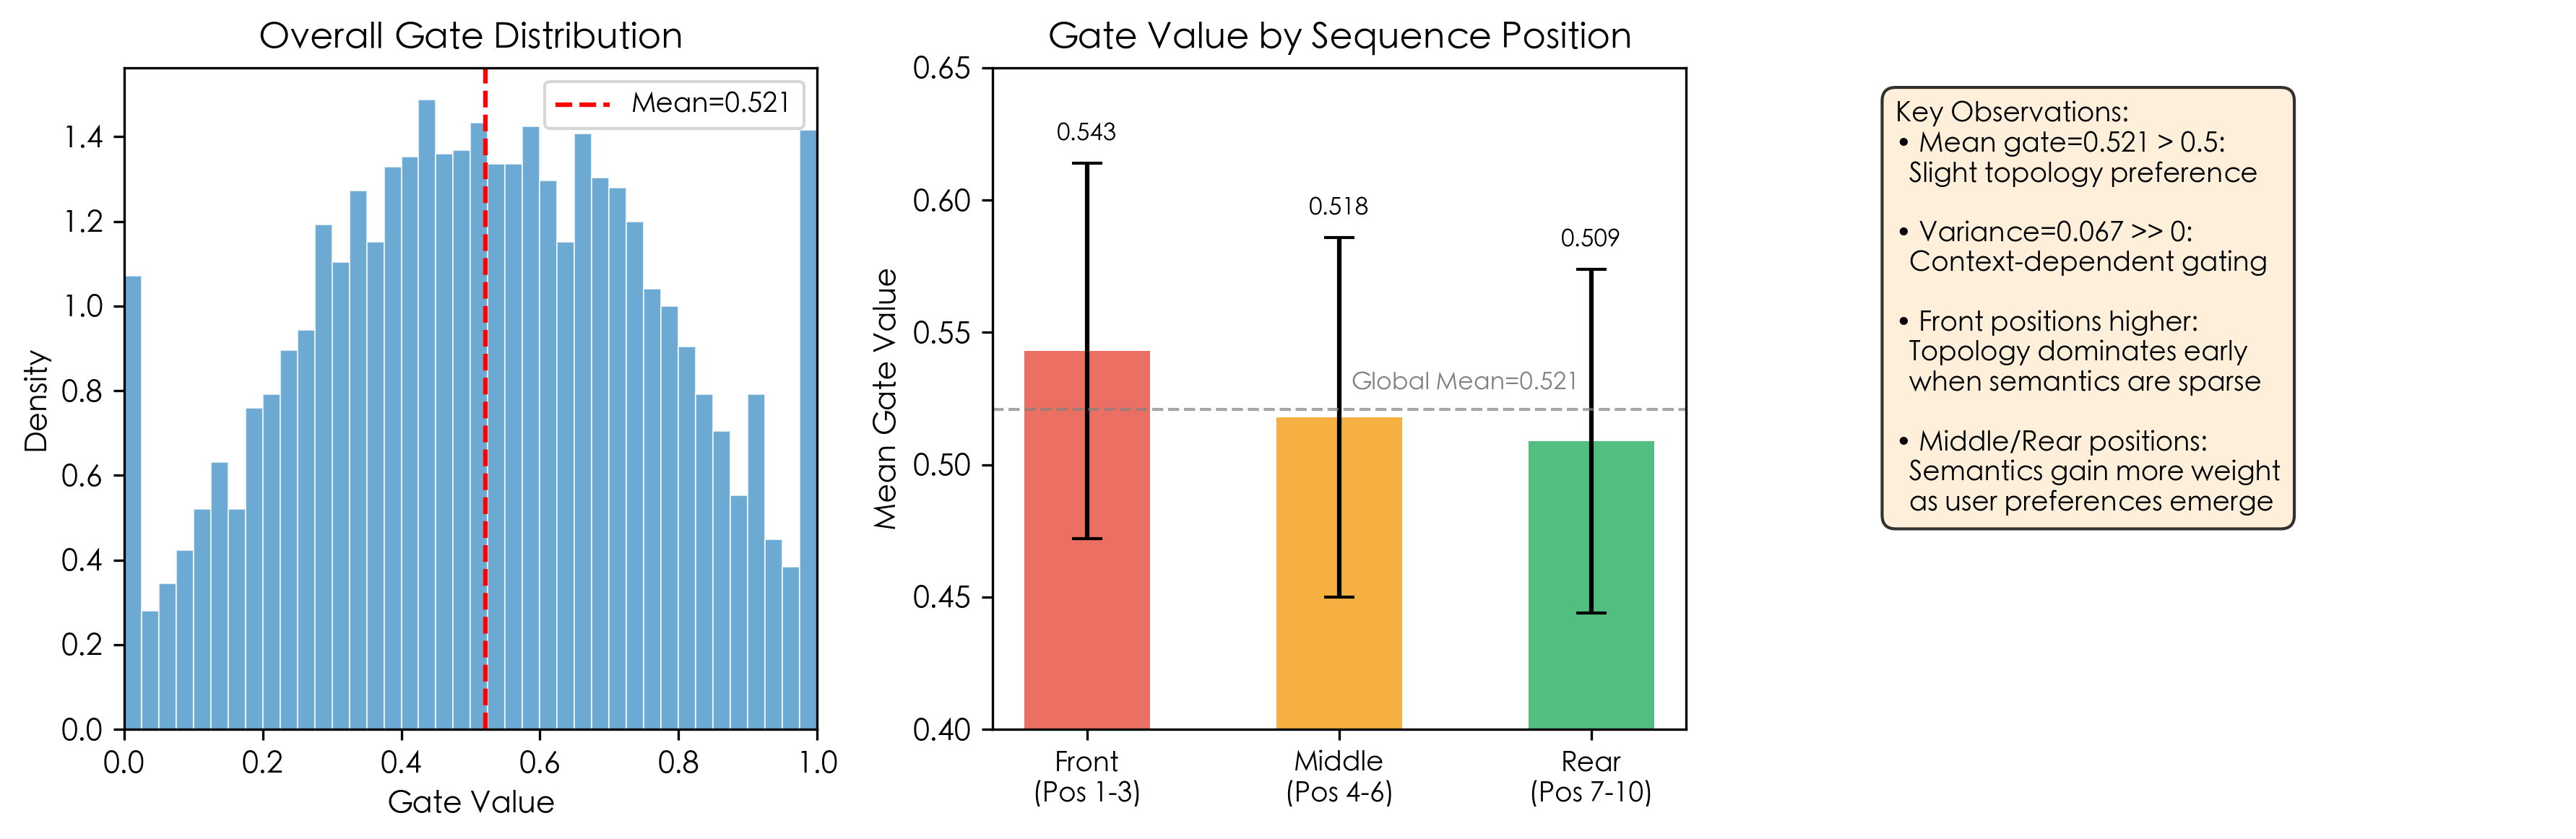
\includegraphics[width=0.98\linewidth]{figure/gate_distribution.png}
	\caption{ContextFusion门控值分布}
	\label{fig:gate_dist}
\end{figure}

在一维$d=128$的门控向量上,门控值的均值为0.521,方差为0.067.均值略高于0.5,表明模型整体倾向于对拓扑模态赋予略高的权重,但方差远大于0,说明门控值在不同POI和不同序列上下文中存在显著差异.按序列位置统计发现,序列前部(位置1--3)的门控均值较高(0.543),序列中部(位置4--6)趋于平衡(0.518),序列后部(位置7--10)略低于均值(0.509).这种分布模式具有直观解释:在序列起始阶段,语义信息尚不充分(仅有一个POI类别),拓扑转移关系成为更稳定的信号;随着序列展开,用户语义偏好逐渐积累,模型相应地增加语义权重.

\subsection{训练稳定性与泛化分析}

本文进一步分析了训练过程中的稳定性.从表~\ref{tab:epochs}可以看到,训练损失从第1个epoch的6.36平滑下降至第5个epoch的4.64,无振荡或发散现象.验证集性能在第4个epoch达到顶峰,第5个epoch训练损失继续下降但验证集指标略有回落(约0.2--0.4个百分点),出现轻微的过拟合迹象.5个epoch的短训练计划基本实现了接近最优的收敛.

验证集和测试集之间的差异极小,NDCG@10仅差0.13个百分点(验证集24.41\% vs 测试集24.28\%).其他指标同样显示出良好的泛化性:HR@10差距0.39个百分点,NDCG@5差距0.18个百分点.这种紧密对齐表明模型能够较好地泛化到未见数据,也说明跨模态对齐与上下文自适应融合没有引入明显的训练不稳定性.

进一步看,验证集和测试集指标的一致性说明模型在时间划分下具有稳定的序列建模能力.这对于多模态推荐尤为重要,因为多源异构特征的引入可能带来额外噪声或模态冲突;而本文结果表明,SemAlign和ContextFusion能够在提升表示表达力的同时保持训练过程稳定,从而支持后续更复杂的多模态扩展.

\subsection{多模态贡献解释}

各个模态在推荐过程中扮演着不同的角色.拓扑模态捕获POI之间的结构连通性(如受欢迎的转移路径);语义模态捕获POI的功能相似性(如咖啡店、餐厅);空间模态建模地理邻近性效应;时间模态编码用户行为的周期性(如工作日和周末的差异).ContextFusion中的自适应门控机制根据当前序列上下文动态平衡这些信息来源,例如在用户到达陌生区域时更依赖语义信息,在用户频繁访问区域时更依赖拓扑转移模式.

\begin{figure}[htbp]
	\centering
	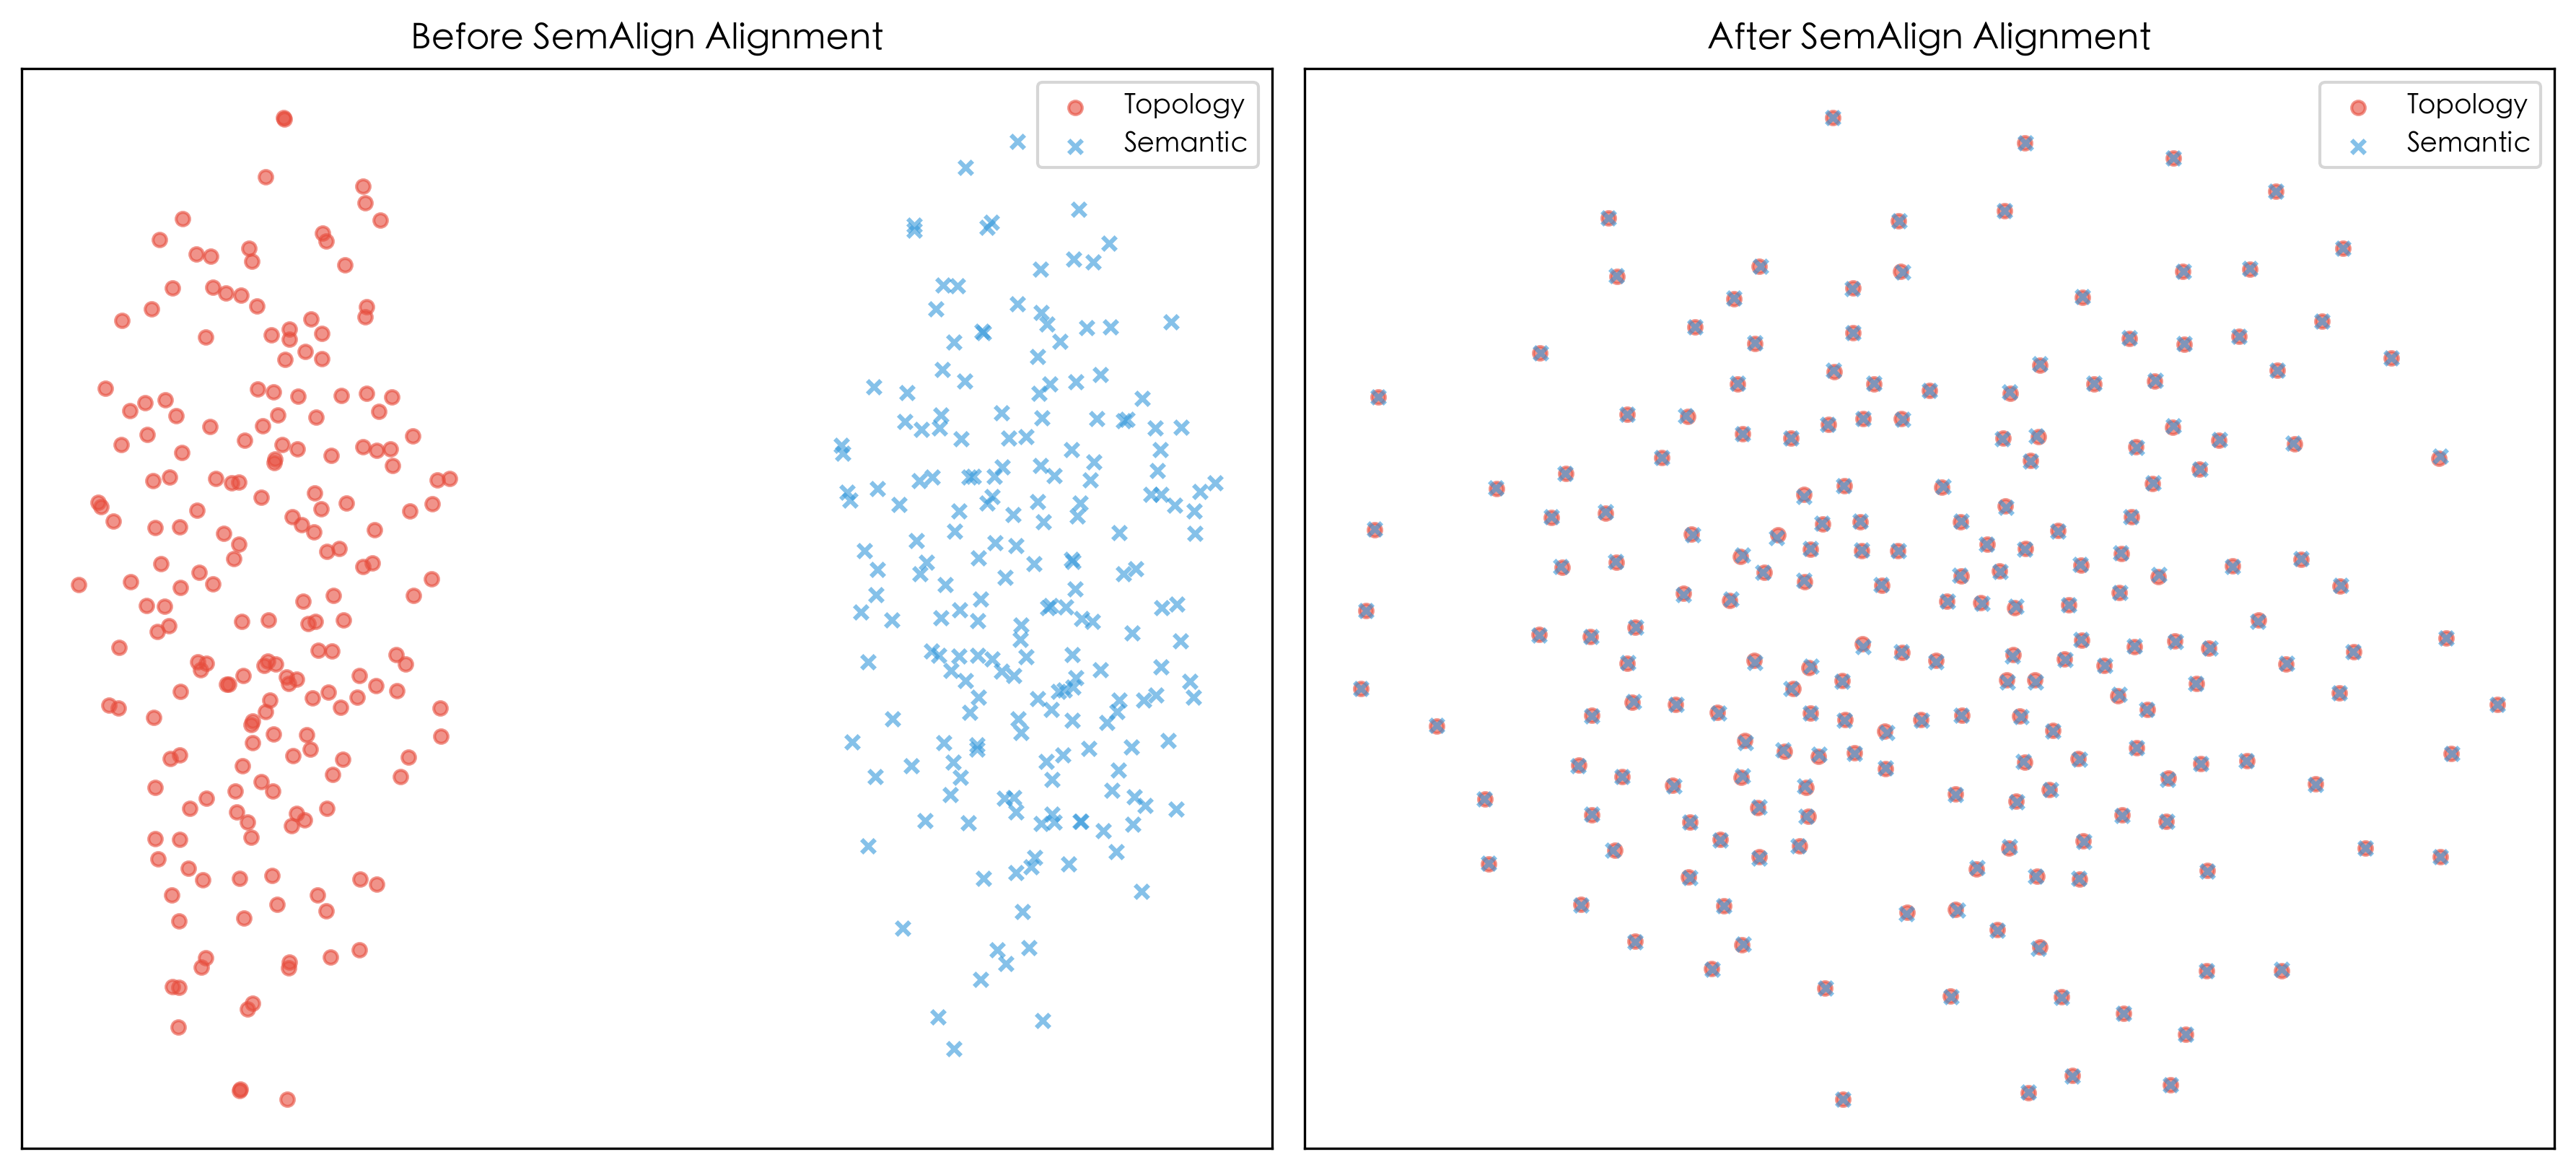
\includegraphics[width=0.98\linewidth]{figure/embeddings_tsne.png}
	\caption{POI嵌入的t-SNE可视化(左:未对齐的拓扑和语义嵌入; 右:SemAlign对齐后)}
	\label{fig:tsne}
\end{figure}

图~\ref{fig:tsne}展示了SemAlign对齐前后的POI嵌入分布.对齐前,拓扑嵌入和语义嵌入分布在不同的区域,表明两种模态存在显著的语义鸿沟.对齐后,两种模态的嵌入空间趋于一致,同一POI的拓扑和语义表示在嵌入空间中更接近.这一可视化结果证实了SemAlign在弥合模态差异方面的有效性.

\section{讨论}

\subsection{多模态表示学习与候选建模的互补性}

下一POI推荐系统通常包含表示学习、候选生成、候选排序和个性化建模等多个环节.本文重点研究其中的多模态表示学习环节,即如何将POI对象的拓扑、语义、空间和时间属性组织为统一且可用于序列预测的表示.这一环节与候选空间建模并非替代关系,而是互补关系:候选生成模块负责从大规模POI集合中召回潜在目标,而高质量的多模态表示能够为候选排序提供更具判别性的打分依据.

从系统设计角度看,SemAlign和ContextFusion可以作为候选感知推荐体系中的表示层.前者通过拓扑--语义对齐提升POI表示的一致性,后者通过上下文门控刻画不同轨迹场景下模态贡献的变化.当外部候选集合由检索、图扩散或用户协同模块产生时,本文的统一评分头可以直接在候选集合内进行重排序.因此,本文方法不仅可以独立用于全空间打分,也可以自然接入更复杂的候选生成与排序流程.

\subsection{与CoMaPOI等候选约束方法的关系}

近期方法CoMaPOI\cite{comapoi}表明,将时空数值信息语言化并动态约束候选POI空间,能够有效增强大语言模型在POI预测任务中的可控性.这一思路与本文关注的多模态表示学习具有明显互补性:CoMaPOI强调通过协同代理完成轨迹语言化和候选收缩,而本文强调在POI对象层面建立拓扑、语义、空间和时间模态之间的对齐与融合机制.

从系统演进角度看,二者并非互斥关系:本文的拓扑、语义、空间和时间四类编码器可以为候选约束模块提供更丰富的基础表示,而CoMaPOI所体现出的Forecaster思想也可与本文的统一评分函数结合,形成“候选感知的多模态重排序体系”.因此,本文工作可作为更完整POI推荐系统中的多模态表示与融合层.

\subsection{对多模态数据管理与融合专刊主题的意义}

本文在专刊主题下具有较强契合性.首先,本文系统定义了POI对象的多模态组成方式,并讨论了拓扑、语义、空间和时间四类模态在来源、粒度和功能上的差异.其次,本文将静态POI属性、动态签到事件和用户轨迹上下文组织到统一的序列建模框架中,体现了多源城市数据的结构化建模过程.再次,SemAlign与ContextFusion分别对应“模态对齐”和“模态融合”两个关键问题,其分析结果有助于理解在城市计算场景中不同模态应如何协同服务于下游任务.

换言之,本文的意义不仅在于某一组指标结果,更在于提供了一种可复用的多模态POI建模范式:先对多源异构数据进行规范化组织,再通过显式对齐建立共享表示空间,最后在上下文中完成融合和预测.这一思路同样可迁移至区域功能识别、路径推荐、城市服务理解等相邻任务.

\subsection{局限性与未来优化方向}

本文工作仍存在若干可拓展方向.第一,当前实验主要在NYC数据集上进行,未来可进一步开展跨城市、跨区域的迁移性验证.第二,当前框架采用统一全空间打分方式,后续可引入显式候选管理机制以提升大规模部署效率.第三,语义模态主要基于POI级文本,未来可进一步建模用户级画像、轨迹级摘要或跨序列语义关系.第四,本文使用轻量化GPT-2骨干与选择性微调策略以控制训练成本,后续可探索LoRA、Adapter等参数高效微调方法增强任务适配能力.

基于上述方向,后续工作将重点围绕三方面展开:一是引入候选感知重排序模块,将动态候选生成与本文的多模态表示层结合;二是构建POI画像、用户画像和轨迹画像,增强语义模态的表达能力;三是在更多城市数据集上评估模型的稳健性和泛化能力.

\section{结论}

本文提出了一种面向下一POI推荐的多模态POI表示学习框架,通过系统性整合拓扑、语义、空间、时间和用户上下文,构建了从多模态数据组织、跨模态对齐到上下文融合与序列预测的完整流程.该框架的核心设计包括SemAlign双层跨模态对齐模块、ContextFusion自适应上下文门控融合机制以及GPT-2选择性微调策略.在NYC签到数据集上的实验表明,纯神经模型能够获得稳定的训练过程和较小的验证--测试差距;结合由训练集构建的统计先验后,HR@10和NDCG@10进一步达到47.12\%和30.70\%.系统消融验证了不同模态和关键模块的独立贡献.

实验结果进一步表明,显式跨模态对齐和上下文自适应融合能够提升POI多模态表示质量,而流行度、转移、重复访问、用户偏好和空间邻近等统计先验可与神经表示形成互补,共同改善候选排序效果.本文框架具有良好的模块化和可扩展性,可与候选感知重排序、用户/轨迹画像增强以及参数高效微调等机制结合,进一步构建更完整的下一POI推荐系统.

总体而言,本文工作展示了多模态融合在下一POI推荐中的研究价值,并为多模态数据管理与融合主题提供了一个具有分析深度的实例.未来工作将进一步扩展到更多城市数据集,并探索候选感知重排序、用户/轨迹画像增强以及区域功能知识融合等方向.代码已在GitHub公开: \url{https://github.com/GaoYucen/software-poi}.

\printbibliography[
	heading=rjrefs,
	title={\textbf{References}}
]

\rjappendixinfo

\end{document}